\documentclass[14pt]{article}

\usepackage[utf8x]{inputenc}
\usepackage[russian]{babel}
\usepackage{graphicx}
\graphicspath{{images/}}
\DeclareGraphicsExtensions{.pdf,.png,.jpg}

\usepackage{amsmath}
\usepackage{pgfplots}

\usepackage{geometry} % Меняем поля страницы
\geometry{left=2cm}% левое поле
\geometry{right=1.5cm}% правое поле
\geometry{top=2cm}% верхнее поле
\geometry{bottom=2cm}% нижнее поле

\renewcommand{\theenumi}{\arabic{enumi}}
\renewcommand{\labelenumi}{\arabic{enumi}}
\renewcommand{\theenumii}{.\arabic{enumii}}
\renewcommand{\labelenumii}{\arabic{enumi}.\arabic{enumii}.}
\renewcommand{\theenumiii}{.\arabic{enumiii}}
\renewcommand{\labelenumiii}{\arabic{enumi}.\arabic{enumii}.\arabic{enumiii}.}

\begin{document}
\begin{titlepage}
	\begin{center}
		\fontsize{18pt}{20pt}\selectfont
		\textbf{Работа 3.2.4.}	
	
		\vspace{5cm}
		\fontsize{24pt}{25pt}\selectfont
		Свободные колебания в электрическом контуре
	\end{center}
	\begin{flushright}
		\fontsize{18pt}{20pt}\selectfont
		\vspace{14cm}
		\hspace{-3cm}
		\textit{Корнеев Е.С.}
	\end{flushright}		
\end{titlepage}

\begin{center}
	\fontsize{16pt}{18pt}\selectfont	
	Свободные колебания в электрическом контуре
\end{center}


\fontsize{14pt}{16pt}\selectfont
\vspace{1cm}
\textbf{Цель работы:} исследование свободных колебаний в колебательном контуре.

\vspace{0.5cm}
\textbf{Оборудование:} генератор импульсов, электронное реле, магазин сопротивлений, магазин ёмкостей, индуктивность, элекронный осциллограф, универсальный мост. 

\vspace{1cm}
Исследуемый колебательный контур состоит из индуктивности $L$, емкости $C$ и резистора $R$. Конденсатор заряжается короткими одиночными импульсами, после каждого из которых в контуре возникают свободные затухающие колебания. Снимая осциллографом напряжение с конденсатора, можно определить основые характеристики цепи. Схема установки для изучения затухающих колебаний изображена на рис. 1:

\begin{figure}[h!]
	\center{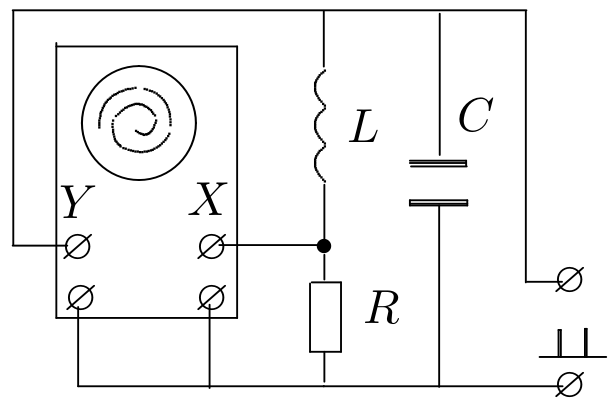
\includegraphics[width = 10cm]{scheme1}}
	\caption{Схема установки}
	\label{fig:image}
\end{figure}

\textbf{Экспериментальная установка.} На рис. 2 приведена схема для исследования свободных колебаний в $RLC$-контуре. Колебаний наблюдаются на экране осциллографа. Для периодического возбуждения колебаний в контуре используется генератор импульсов Г5-54. С выхода генератора по коаксиальному кабелю импульсы поступают через электронное реле,смонтированное в отдельном блоке. Реле содержит диодный тиристор $D$ и ограничительный резистор $R_1$. 

\begin{figure}[h!]
	\center{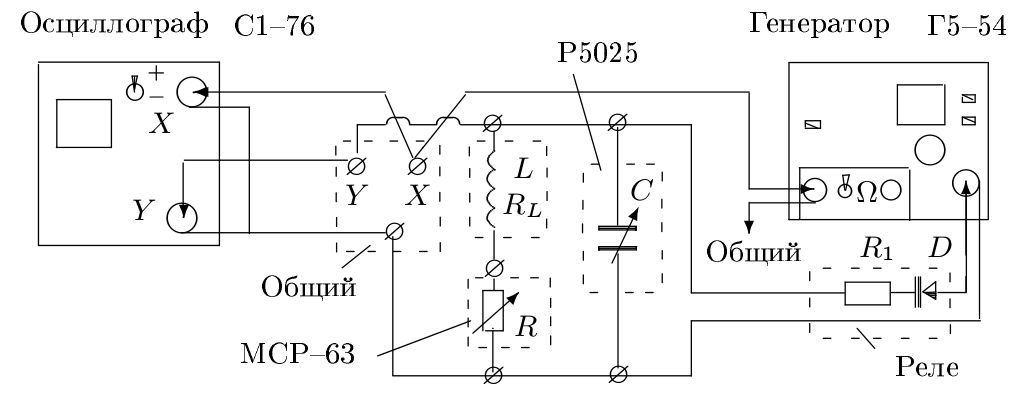
\includegraphics[width = 15cm]{scheme2}}
	\caption{Схема установки}
	\label{fig:image}
\end{figure}

Импульсы заряжают конденсатор $C$. После каждого импульса генератор отключается от колебательного контура, и в контуре возникают свободные затухающие колебания. Входное сопротивление осциллографа велико ($\approx 1$МОм), так что его влиянием на контур можно пренебречь. Для получения устойчивой картины затухающих колебаний используется режим ждущей развертки с синхронизацией внешними импульсами, поступающими с выхода "синхроимпульсы" генератора. 

\vspace{1cm}
\textbf{Ход работы.}

0. Измерим индуктивность катушки и ее сопротивление в зависимости от частоты:

\begin{center}
\begin{tabular}{|c|c|c|c|c|c|c|c|c|c|c|}
\hline
$L$, мГн	&	$R$, Ом		&	$f$, Гц		\\
\hline
144			&	10.3		&	0.050		\\
\hline
139			&	11.3		&	1000		\\
\hline
140			&	13.0		&	5000		\\
\hline
\end{tabular}
\end{center}

Откуда сразу получим, что $L = (141 \pm 2)$мГн, $R = (11.5 \pm 1)$Ом.

\vspace{1cm}

1. Установим значение сопротивления $R = 0$ и емкости $C = 0.02$ мкФ, после чего прокалибруем осциллограф, зная частоту синхронизирующего сигнала $\nu = 100$Гц 
($T_0 = 0.01$c): в выбранном масштабе ему соответствует $x_0$ = 50 делений, то есть $1\text{дел} = 0.0002$c. Теперь, зная цену деления, определим зависимость периодов колебаний от емкости $C$ по осциллограмме. Формула, которой мы пользуемся, имеет вид
$$
	T_{\text{эксп}} = T_0\frac{x}{nx_0},
$$
\noindent где $n$ - число полных периодов. Теоретическое же значение получим по формуле
$$
	T_{\text{теор}} = 2\pi\sqrt{LC},
$$
\noindent зная, что $L = 140$ мГн.

\begin{center}
\begin{tabular}{|c|c|c|c|c|c|c|c|c|c|c|c|}
\hline
$n$&$x$, дел&С, мкФ&$T_{\text{эксп}}$, мс&$\sigma_{эксп}$, мс&$T_{\text{теор}}$, мс&$\sigma_{теор}$, мс\\
\hline
30&50&0,02&0,33&0,02&0,33&0,00\\
\hline
14&50&0,10&0,71&0,04&0,74&0,01\\
\hline
9&48&0,20&1,07&0,06&1,05&0,01\\
\hline
8&50&0,30&1,25&0,08&1,29&0,02\\
\hline
7&50&0,40&1,43&0,09&1,49&0,02\\
\hline
5&42&0,50&1,68&0,08&1,66&0,02\\
\hline
5&46&0,60&1,84&0,11&1,82&0,03\\
\hline
4&40&0,70&2,00&0,12&1,97&0,03\\
\hline
4&43&0,80&2,15&0,13&2,10&0,03\\
\hline
4&46&0,90&2,30&0,14&2,23&0,03\\
\hline
\end{tabular}

\end{center}

Оценим погрешности: $\sigma_x$ примем равной 1 дел, так как нельзя точно определить эту величину из-за толщины линии. Погрешность $\sigma_{x_0}$ примем равной 2 дел из-за сложности определения начала и конца импульса. Погрешность $n$ отсутствует, а погрешностью $C$ можно пренебречь на фоне остальных погрешностей. Тогда погрешность величины 
$T_{\text{эксп}}$ определим по формуле
$$
	\sigma_{приб} = \sqrt{\sum_{i = 1}^n \left(\frac{\partial f}{\partial x_i}\sigma_i\right)^2},
$$
\noindent считая $T_{\text{эксп}} = f(x, x_0)$. Погрешность теоретического значения получим по этой же формуле, считая $T_{\text{теор}} = f(L)$.

Теперь можно построить график $T_{\text{эксп}} = f(T_{\text{теор}})$:

\begin{tikzpicture}
\begin{axis}[
	height = 10cm,
	width  = 15cm,
	every axis y label/.style={at = {(ticklabel cs: 0.5)}, rotate = 90, anchor = near ticklabel},
	xlabel = {$T_{\text{теор}}$, мс},
	ylabel = {$T_{\text{эксп}}$, мс},
	grid   = major,
	ymin  = 0,
	xmin  = 0.2
]
\addplot+[
	only marks,
	error bars/.cd, 
	y dir = both, y explicit,
	x dir = both, x explicit,
	]
coordinates{
	(0.33, 0.33)	+-	(0.00, 0.02)
	(0.74, 0.71)	+-	(0.01, 0.04)
	(1.05, 1.07)	+-	(0.01, 0.06)
	(1.29, 1.25)	+-	(0.02, 0.08)
	(1.49, 1.43)	+-	(0.02, 0.09)
	(1.66, 1.68)	+-	(0.02, 0.08)
	(1.82, 1.84)	+-	(0.03, 0.11)
	(1.97, 2.00)	+-	(0.03, 0.12)
	(2.10, 2.15)	+-	(0.03, 0.13)
	(2.23, 2.30)	+-	(0.03, 0.14)
};

\addplot [mark = none, color = blue]
coordinates{
	(0.33, 0.29475)
	(2.23, 2.26696)
};

\end{axis}
\end{tikzpicture}

\vspace{1cm}
2. Рассчитаем значение $C$, для которого реализуется $\nu = 5$кГц в предположении, что $L = 200$мГн:
$$
	C = \frac{1}{(2\pi\nu)^2L} = 0.005\text{мкФ},
$$
\noindent чему соответствует $R = 2\sqrt{L/C} = 12650$ Ом. Экспериментально определим $R_{\text{кр}} = 8$кОм. Определим логарифмический декрмемент затухания по формуле
$$
	\Theta = \frac{1}{n}\ln\frac{U_k}{U_{k + n}},
$$
\noindent где $U_k$ и $U_{k+n}$ - амплитуды $k$-го и $k+n$-го периода.

\begin{center}
\begin{tabular}{|c|c|c|c|c|c|c|c|c|c|}
\hline
$n$&$U_1$, дел&$U_2$, дел&$R$, Ом&$R_{\text{конт}}$, Ом&$\Theta$&$\sigma_{\Theta}$\\
\hline
5&10&1&800&812&0,46&0,06\\
\hline
5&20&1&1000&1012&0,60&0,05\\
\hline
4&14&1&1200&1212&0,66&0,06\\
\hline
3&11&1&1400&1412&0,80&0,08\\
\hline
3&15&1&1600&1612&0,90&0,08\\
\hline
2&20&2&1800&1812&1,15&0,06\\
\hline
2&13&1&2000&2012&1,28&0,12\\
\hline
2&22&1&2200&2212&1,55&0,11\\
\hline
1&21&3&2400&2412&1,95&0,09\\
\hline
\end{tabular}

\end{center}

Для оценки погрешности воспользуемся тем, что магазин сопротивлений позволяет выставить $R$ с высокой тоностью, поэтому погрешность $R_{\text{конт}}$ примем равной погрешности $R_L$, которая в свою очередь равна $\pm 1$ Ом. Погрешность амплитуды $U_1$ будет $\sigma_{U_1} = 0.5$ дел. Также примем погрешность $\sigma_{U_2}$ равной 
$0.2$ дел., оценив толщиной линии, так как очевидно, что в данном случае мы хорошо видим снимаемую величину на экране, а также при измерениях мы специально выбирали те колебания, чья амплитуда была наиболее точно попадавшей на деления. Отдельно стоит отметить, что из-за того, что изображение на экране осциллографа не было статичным, стоило выбирать удаленные амплитуды, чтобы минимизировать ошибку, вызванную случайными движениями. Погрешность $\sigma_n$ равна 0. Погрешность $\sigma_{\Theta}$ определим по уже известной формуле, считая $\Theta = f(U_1, U_2)$.

Теперь построим зависимость $1/\Theta^2 = f(1/R_{\text{конт}}^2)$. Погрешность $\sigma_{1/R^2}$ пренебрежимо мала, погрешность $\sigma_{1/\Theta^2}$ определим, зная, что 
$\varepsilon_{1/\Theta^2} = 2\varepsilon_{\Theta}$:

\begin{center}
\begin{tabular}{|c|c|c|c|c|c|}
\hline
$1/R_{\text{конт}}^2$, Ом$^-2 \cdot 10^{-6}$&$1/\Theta^2$&$\sigma_{1/\Theta^2}$\\
\hline
1,52&4.7&0,6\\
\hline
0,98&2,8&0,5\\
\hline
0,68&2,3&0,4\\
\hline
0,50&1,6&0,3\\
\hline
0,38&1,2&0,2\\
\hline
0,30&0,8&0,1\\
\hline
0,25&0,6&0,1\\
\hline
0,20&0,4&0,1\\
\hline
0,17&0,3&0,0\\
\hline
\end{tabular}
\end{center}

\vspace{1cm}
Теперь можно построить график $1/\Theta^2 = f(1/R_{\text{конт}}^2)$:

\vspace{1cm}
\begin{tikzpicture}
\begin{axis}[
	height = 10cm,
	width  = 15cm,
	every axis y label/.style={at = {(ticklabel cs: 0.5)}, rotate = 90, anchor = near ticklabel},
	xlabel = {$1/R_{\text{конт}}^2$, Ом$^-2 \cdot 10^{-6}$},
	ylabel = {$1/\Theta^2$},
	grid   = major,
	ymin   = 0,
	xmin   = 0
]
\addplot+[
	only marks,
	error bars/.cd, 
	y dir = both, y explicit,
	x dir = both, x explicit,
	]
coordinates{
	(1.52, 4.7)		+-	(0, 0.6)
	(0.98, 2.8)		+-	(0, 0.5)
	(0.68, 2.3)		+-	(0, 0.4)
	(0.50, 1.6)		+-	(0, 0.3)
	(0.38, 1.2)		+-	(0, 0.2)
	(0.30, 0.8)		+-	(0, 0.1)
	(0.25, 0.6)		+-	(0, 0.1)
	(0.20, 0.4)		+-	(0, 0.1)
	(0.17, 0.3)		+-	(0, 0.0)
};

\addplot [mark = none, color = blue]
coordinates{
	(1.52, 4.72431)
	(0.17, 0.4076)
};

\end{axis}
\end{tikzpicture}

Из графика по МНК определим $(\Delta 1/\Theta^2)/(\Delta 1/R^2)$:
$$
	\frac{\Delta 1/\Theta^2}{\Delta 1/R^2} = 3.2 \cdot 10^6 \text{Ом}^2
$$
Также по МНК определим случайную погрешность $(\Delta 1/\Theta^2)/(\Delta 1/R^2)$:
$$
	\sigma_{\frac{\Delta 1/\Theta^2}{\Delta 1/R^2}_\text{случ}} = 0.4 \cdot 10^6 \text{Ом}^2
$$
Считая $\frac{\Delta 1/\Theta^2}{\Delta 1/R^2} = f(1/\Theta^2, 1/R^2)$, определим приборную погрешность:
$$
	\sigma_{\frac{\Delta 1/\Theta^2}{\Delta 1/R^2}_\text{приб}} = 0.5 \cdot 10^6 \text{Ом}^2
$$
Теперь можно определить полную погрешность по формуле
$$
	\sigma_{\text{полн}} = \sqrt{\sigma_{\text{случ}}^2 + \sigma_{\text{приб}}^2}
$$
Откуда
$$
	\frac{\Delta 1/\Theta^2}{\Delta 1/R^2} = (3.2 \pm 0.6) \cdot 10^6 \text{Ом}^2
$$

Теперь можно определить $R_{\text{кр, граф}}$ по формуле
$$
	R_{\text{кр, граф}} = 2\pi\sqrt{\frac{\Delta 1/\Theta^2}{\Delta 1/R^2}}:
$$
$$
	R_{\text{кр, граф}} = (11 \pm 1)\cdot10^3 \text{Ом}
$$

Таким образом, мы видим следующую картину:
$$	
	R_{\text{кр, теор}} = 12 \text{кОм},~~R_{\text{кр, граф}} = 11 \text{кОм},~~R_{\text{кр, прак}} = 8 \text{кОм}
$$
Как и ожидалось, теоретическое значение $R$ совпадает с графическим в пределах погрешности, однако практическое значение оказалось несколько меньше, чем рассчетные, что связано в частности с тем, что предполагаемое значение $L$ достаточно сильно отличается от реального.

\vspace{1cm}
3. Определим значения $Q_{\text{прак}}$ по формуле $Q_{\text{прак}} = \pi/\Theta$, и $Q_{\text{теор}}$ по формуле $Q_{\text{теор}} = \frac{1}{R}\sqrt{\frac{L}{C}}$:

\begin{center}
\begin{tabular}{|c|c|c|c|c|c|c|c|}
\hline
$~~~\Theta~~~$	&	$~~~Q_{\text{прак}}~~~$	&	$~~~Q_{\text{теор}}~~~$		\\
\hline
0.46			&	6.83					&	6.52						\\
\hline
1.95			&	1.61					&	2.19						\\
\hline
\end{tabular}
\end{center}

Полученные экспериментально значения отличаются от теоретических, так как теоретическое значение получено в предположении малых затуханий, однако в нашем случае затухания таковыми считать можно не всегда. Видно, что при уменьшении активного сопротивления теоретическое значение приближается к полученному экспериментально.

\vspace{1cm}
4. Определим $\Theta$ по спирали:

\begin{center}
\begin{tabular}{|c|c|c|c|c|c|c|c|c|}
\hline
$n$&$U_1$, дел&$U_2$, дел&$R$, Ом&$R_{\text{конт}}$, Ом	&$\Theta$	\\
\hline
4&24&3&800&812&0,52\\
\hline
4&29&2&1000&1012&0,67\\
\hline
1&29&6&2200&2212&1,58\\
\hline
1&23&4&2400&2412&1,75\\
\hline
\end{tabular}
\end{center}

Сравнивая значения $\Theta$ с полученными экспериментально в пункте 3, получим, что они близки, чего и следовало ожидать.

\vspace{1cm}
Таким образом, в данной лабораторной работе мы изучили поведение колебательного $RLC$-контура в зависимости от величины активного сопротивления. Изучая затухающие колебания, периодически возбуждаемые в цепи импульсами, мы определили добротность контура и сравнили значения, полученные экспериментально, со значениями, полученными по рассчетным формулам. Из результатов видно, что результаты тем лучше описываются теоретически, чем меньше активное сопротивление цепи.

\end{document}